\documentclass{beamer}
\usepackage[utf8]{inputenc}
\usepackage{graphicx}
\usepackage[ngerman]{babel}
\usepackage[T1]{fontenc}
% enthält die konfiguration für das listings package
\usepackage{listings}
\usepackage{xcolor}
\lstset{language=Java}
\definecolor{lst_light_grey}
{rgb}{0.95,0.95,0.95}
\definecolor{lst_dark_grey}
{rgb}{0.8,0.8,0.8}
\definecolor{lst_highlight}
{rgb}{0,0,0.6}
\definecolor{lstgreen}
{rgb}{0,0.6,0}
\definecolor{lstmauve}
{rgb}{0.58,0,0.82}
\lstset{ %
basicstyle=\small\ttfamily, %
backgroundcolor=\color{lst_light_grey}, %
captionpos=b, %
commentstyle=\color{lstgreen}, %
frame=single, %
tabsize=2, %
%
keywordstyle=\color{lst_highlight}, %
%
numbers=left, %
%
numberstyle=\scriptsize \color{lst_dark_grey}, %
%
rulecolor=\color{lst_dark_grey}, %
}
% additional highlighted keywords
\lstset { emph= {%
var, function %
}, emphstyle={\color{lst_highlight}}%
}
\lstset{showstringspaces=false}

\author{Marlene Knoche}
\title{\LaTeX-Seminar}
\begin{document}

\begin{frame}

\maketitle

\end{frame}

\begin{frame}

\tableofcontents

\end{frame}

\section{Was ist \LaTeX?}

\begin{frame}
\centering
\huge{Was ist \LaTeX?}
\end{frame}

\begin{frame}{Geschichte - I}
\begin{itemize}
\item Ursprünglich wurde \TeX\; von Donald E. Knuth entwickelt
\item \LaTeX\; ist Sammlung von \TeX-Makros von Leslie Lamport 
\end{itemize}

\begin{figure}
\centering
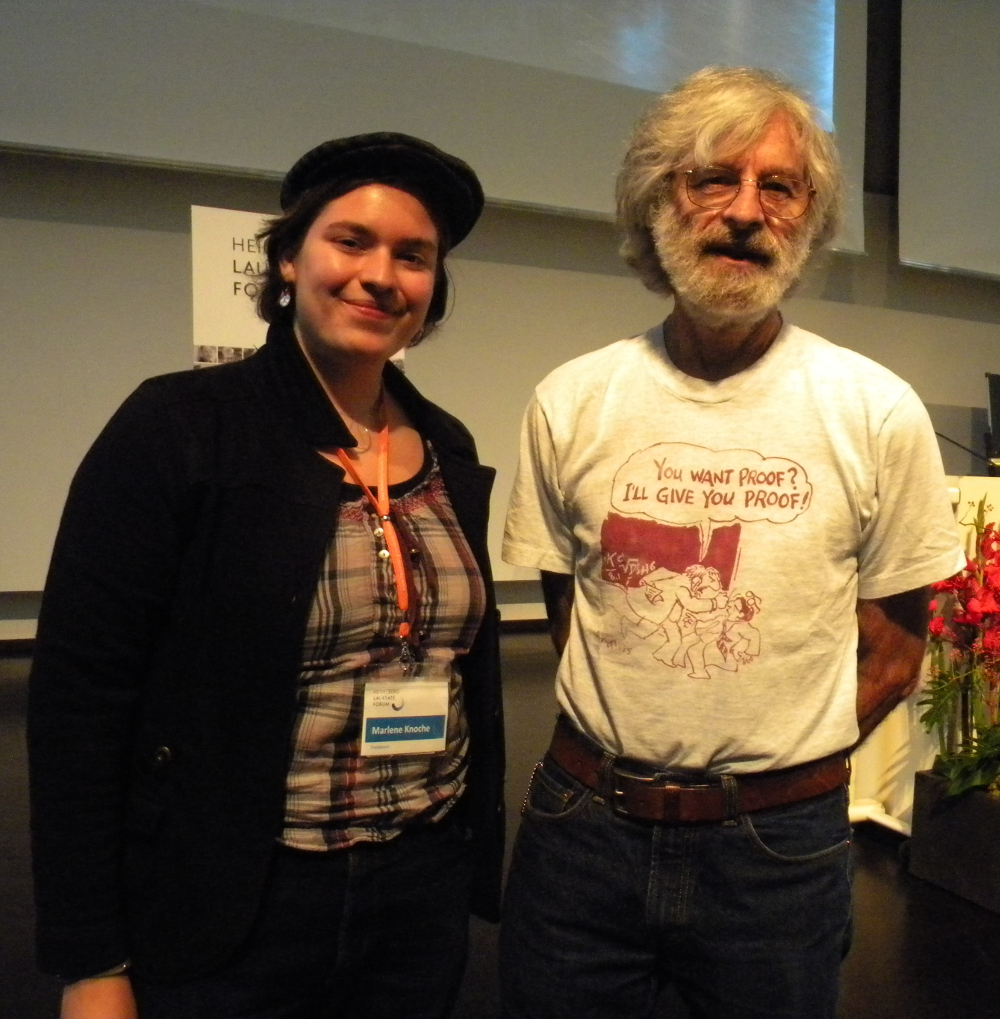
\includegraphics[scale=0.5]{pics/leslielamport.jpg}
\caption{Leslie Lamport und ich in Heidelberg beim HLF14 2014}
\end{figure}
\end{frame}

\begin{frame}{Geschichte - II}
\begin{itemize}
\item Entwicklung 1990 von Lamport eingestellt
\item Seit 1989 ist \LaTeX $2_{\varepsilon}\;$ von Frank Mittelbach, Chris Rowley und Rainer Schöpf weiter entwickelt worden
\item Seit Mitte der 1990er ist \LaTeX $2_{\varepsilon}\;$ am weitesten verbreitete Methode, \TeX\; zu nutzen
\end{itemize}
\end{frame}

\begin{frame}{WYSIWYG vs WYGIWYM}

\begin{block}{WYSIWYG}
= \textbf{W}hat \textbf{y}ou \textbf{s}ee \textbf{i}s \textbf{w}hat \textbf{y}ou \textbf{g}et

Formatierung wird direkt angezeigt
\end{block}

\begin{block}{WYGIWYM}
= \textbf{W}hat \textbf{y}ou \textbf{g}et \textbf{i}s \textbf{w}hat \textbf{y}ou \textbf{m}ean

Formatierung wird beschrieben
\end{block}

\begin{itemize}
\item \LaTeX \; ist Vertreter für WYGIWYM
\end{itemize}
\end{frame}

\begin{frame}{Betriebssysteme und Editoren}

\begin{itemize}
\item Editoren und \LaTeX-Umgebung für alle Plattformen verfügbar
\item TeXworks standardmäßig bei Installation dabei (alle Plattformen)
\item Andere Editoren: 
	\begin{itemize}
	\item TeXlipse Plugin für Eclipse (alle Plattformen)
	\item Texmaker (alle Plattformen
	\item TeXstudio (alle Plattformen)
	\item Kile (KDE(Linux), Windows)
	\item TeXnicCenter (Windows)
	\item \ldots
	\end{itemize}
\end{itemize}

\end{frame}

\section{Grundlegendes}
\begin{frame}
\centering
\huge{Grundlegendes}
\end{frame}


\begin{frame}[fragile]{Syntax}

\begin{itemize}
\item Groß- und Kleinschreibung ist relevant!
\item Kommentare beginnen mit \%-Zeichen.
\end{itemize}

\begin{block}{Befehle:}

\begin{itemize}
\item $\backslash$\texttt{Befehlsname}
\item $\backslash$\texttt{Befehlsname}\{\texttt{Option}\}
\item $\backslash$\texttt{Befehlsname}[\texttt{Option}]\{\texttt{Option}\}
\end{itemize}
\end{block}

\begin{block}{Umgebungen:}
\begin{verbatim}
	\begin{Umgebungsname}
	Text und/oder Befehle
	\end{Umgebungsname}
\end{verbatim}

Umgebungen müssen immer geschlossen werden.

Zusätzliche Optionsplatzhalter sind möglich.

\end{block}


\end{frame}

\begin{frame}[fragile]{Grundstruktur Dokument}
\begin{enumerate}
\item Definition einer Dokumentenklasse
	\begin{itemize}
		\item \begin{verbatim}\documentclass[Option]{Dokumentenklasse}\end{verbatim}
		\item z.B. article (scrartcl in KOMA-Script), report (srcreprt in KOMA-Script)
	\end{itemize}
\item Packages nachladen und Konfiguration des Dokumentes
	\begin{itemize}
		\item Packages laden: \begin{verbatim}\usepackage[Option]{Packagename}\end{verbatim}
		\item Angabe von Meta-Informationen wie Autor oder Titel
	\end{itemize}
\item Dokumenteninhalt innerhalb der \texttt{document}-Umgebung
	\begin{itemize}
	\item \begin{verbatim} \begin{document} Text und Befehle \end{document}
	\end{verbatim}
	\end{itemize}
\end{enumerate}
\end{frame}

\begin{frame}[fragile]{Minimalbeispiel}

Minimalistisches Beispiel ohne Packages.

\begin{verbatim}
	\documentclass{article}
	\begin{document}
	\section{Hallo Welt!}
	Ich bin der tolle Text auf der ersten Seite!
	\end{document}
\end{verbatim}
\end{frame}

\begin{frame}[fragile]{Empfohlene Packages}

Packages, die Dokument auf Deutsch umstellen und Sonderzeichen wie ä, ö, ß erlauben.

\begin{verbatim}
\usepackage[utf8]{inputenc}
\usepackage[ngerman]{babel}
\usepackage[T1]{fontenc}
\end{verbatim}
\end{frame}

\section{Dokument}
\begin{frame}
\centering
\huge{Dokument}
\end{frame}

\begin{frame}[fragile]{Gliederungsebenen}
\begin{itemize}
\item Mögliche Gliederungsebenen abhängig von verwendeter Dokumentenklasse
\item section, subsection und subsubsection in allen Dokumentenklassen verfügbar
\item weitere Ebenen: part, chapter (der section übergeordnet, Dokumentenklasse report), paragraph und subparagraph (der subsubsection zugeordnet)
\item Syntax jeweils \begin{verbatim} \gliederungsebene{Name} \end{verbatim}
\item Beispiel siehe Minimalbeispiel
\item $\backslash$\texttt{appendix} leitet den Anhang ein 
\end{itemize}
\end{frame}

\begin{frame}[fragile]{Text formatieren - I}
\begin{itemize}
\item \textbf{fett}: \begin{verbatim}\textbf{fett}\end{verbatim}
\item \textit{kursiv}:\begin{verbatim}\textit{kursiv}\end{verbatim}
\item \texttt{Schreibmaschine}: \begin{verbatim}\texttt{Schreibmaschine}\end{verbatim}
\item {\rmfamily \scshape Kapitälchen}: \begin{verbatim}\textsc{Kapitälchen}\end{verbatim}
\end{itemize}
\end{frame}

\begin{frame}[fragile]{Text formatieren - II}

\begin{itemize}
\item Zusätzlich können Texte durch Befehle besonders klein oder groß dargestellt werden
\item Befehle in aufsteigender Reihenfolge der Größe (Groß- und Kleinschreibung ist relevant!):
\item[] \begin{verbatim} \tiny, \scriptsize, \footnotesize, \small,
 \normalsize, \large, \Large, \LARGE, \huge, 
 \Huge \end{verbatim}
\item[]
\item Zeilenumbrüche über \begin{verbatim}\newline und \\ \end{verbatim}
\item Seitenumbrücke über \begin{verbatim}\newpage\end{verbatim}

\end{itemize}

\end{frame}


\begin{frame}[fragile]{Dokument formatieren - I}

\begin{itemize}
\item Zentrale Layouteinstellungen werden mit der Definition der Dokumentenklasse bestimmt
\item Beispiel: \begin{verbatim}\documentclass[a4paper,11pt, twoside]{scrreprt}\end{verbatim}
\item Ebenfalls in der Präambel können Autor und Titel des Dokumentes bestimmt werden:
\item[] \begin{verbatim} \author{Name} 
\title{Name}\end{verbatim}
\item Titelseite wird über die \texttt{titlepage}-Option bei der Dokumentenklassendefinition oder über den Befehl $\backslash$\texttt{maketitle}  innerhalb der \texttt{document}-Umgebung eingebunden
\end{itemize}

\end{frame}

\begin{frame}[fragile]{Dokument formatieren - II}

\begin{itemize}
\item Alle Arten von Verzeichnissen (Inhalt, Abbildungen, Tabellen, ...) können automatisch generiert werden
\item Zumeist mit nur einem Befehl erzeugbar
\item Befehle: \begin{verbatim}\tableofcontents, \listoffigures, 
\listoftables, \lstlistoflistings \end{verbatim}

\end{itemize}

\end{frame}

\begin{frame}[fragile]{Dokument formatieren - III}

\begin{itemize}

\item Verweise innerhalb des Dokumentes über Labels und Referenzen mittels:
\begin{verbatim} \label{myLabel} \ref{myLabel} \end{verbatim}

\item Numerierung der Seiten in Klein- und Großbuchstaben, arabischen oder römischen Ziffern (klein und groß) möglich:
 \begin{verbatim}\pagenumbering{alph}
\pagenumbering{Alph}
\pagenumbering{arabic}
\pagenumbering{roman}
\pagenumbering{Roman}\end{verbatim}

\end{itemize}
\end{frame}

\begin{frame}[fragile]{Aufzählungen/Listen - I}
\begin{itemize}
\item drei Arten von Aufzählungen: \texttt{itemize} (Stichpunkte), \texttt{enumerate} (Nummerierung), \texttt{description} (Beschreibungen)
\item lassen sich Kombinieren und beliebig verschachteln
\item Syntax: \begin{verbatim} \begin{listenart} \item Inhalt \end{listenart} \end{verbatim}
\end{itemize}
\end{frame}

\begin{frame}[fragile]{Aufzählungen/Listen - II (Beispiel Itemize)}

\begin{minipage}{0.4\textwidth}
\begin{verbatim}
	\begin{itemize}
	\item Stichpunkt 1
	\item[] 42
	\item Neuer Stichpunkt
	\end{itemize}
\end{verbatim}
\end{minipage}
\begin{minipage}{0.4\textwidth}

	\begin{itemize}
	\item Stichpunkt 1
	\item[] 42
	\item Neuer Stichpunkt
	\end{itemize}

\end{minipage}


\end{frame}

\begin{frame}[fragile]{Aufzählungen/Listen - III (Beispiel Enumerate)}

\begin{minipage}{0.4\textwidth}
\begin{verbatim}
	\begin{enumerate}
	\item Stichpunkt 1
	\item [] 42
	\item Neuer Stichpunkt
	\end{enumerate}
\end{verbatim}
\end{minipage}
\begin{minipage}{0.4\textwidth}

	\begin{enumerate}
	\item Stichpunkt 1
	\item [] 42
	\item Neuer Stichpunkt
	\end{enumerate}

\end{minipage}

\end{frame}

\begin{frame}[fragile]{Aufzählungen/Listen - IV (Beispiel Description)}

\begin{minipage}{0.4\textwidth}
\begin{verbatim}
	\begin{description}
	\item [Text] Stichpunkt 1
	\item [Ultimativ] 42
	\item [Neuer] Stichpunkt
	\end{description}
\end{verbatim}
\end{minipage}
\begin{minipage}{0.5\textwidth}

	\begin{description}
	\item [Text] Stichpunkt 1
	\item [Ultimativ] 42
	\item [Neuer] Stichpunkt
	\end{description}

\end{minipage}

\end{frame}

\begin{frame}[fragile]{Grafiken - I}

\begin{itemize}
\item Benötigt das Nachladen eines Packages: \texttt{graphicx} mit \begin{verbatim}\usepackage{graphicx}\end{verbatim}
\item Einbinden einer Grafik selbst: \begin{verbatim} \includegraphics[Option]{Dateiname} \end{verbatim} 
\item Im Optionsbereich wird die Größe des Bilds angegeben
\item Können auch in \texttt{figure}-Umgebung eingebunden werden
\end{itemize}

\end{frame}

\begin{frame}[fragile]{Grafiken - II (Beispiel)}
\begin{verbatim}
	\begin{figure}[h]
	\centering
	\includegraphics[scale=0.5]{Bildname.png}
	\caption{Bildunterschrift}
	\label{fig:Beispielbild}
	\end{figure}
\end{verbatim}
\end{frame}

\begin{frame}[fragile]{Tabellen - I}
\begin{itemize}
\item Können ohne zusätzliches Package verwendet werden
\item Packages vorhanden, die andere Formatierungsmöglichkeiten bieten
\item Syntax: \begin{verbatim} \begin{tabular}[Position]{Spalten} Inhalt \end{tabular} \end{verbatim}
\item Position ist optional
\item kann auch in \texttt{table}-Umgebung eingebettet werden
\item Einzelne Spalteneinträge werden mit \& getrennt
\item Zeilen müssen mit $\backslash \backslash$ abgeschlossen werden, au0er letzter Zeile
\item Auch komplexere Tabellen möglich (Kombination von mehreren Zeilen oder Spalten)
\end{itemize}
\end{frame}

\begin{frame}[fragile]{Tabellen - II (Beispiel Einfache Tabelle)}


\begin{verbatim}
	
\begin{table}
	\begin{tabular}{|l|c|r|}
	\hline
	Text & 1234 & Erste Zeile\\
	\hline
	Hallo & Welt & !\\
	\hline
	\end{tabular}
	\caption{Beispieltabelle}
\end{table}

\end{verbatim}

\begin{table}
	\begin{tabular}{|l|c|r|}
	\hline
	Text & 1234 & Erste Zeile\\
	\hline
	Hallo & Welt & !\\
	\hline
	\end{tabular}
	\caption{Beispieltabelle}
\end{table}
\end{frame}



\begin{frame}[fragile]{Formeln}
\begin{itemize}
\item Einbinden von Formeln in Matheumgebung auch ohne zusatzpackage möglich
\item Für manche Anwendungsfälle jedoch Zusatzpaket z.B. \texttt{amsmath} erforderlich
\item Inline über zwei einschließende \$-Zeichen bzw.d \begin{verbatim}\( ... \)\end{verbatim}
\item Beispiel: \begin{verbatim} \( E = m * c^2 \)\end{verbatim}
\item[] \(E=m*c^2\)
\item Abgesetzt als Block über: \begin{verbatim} \[ ... \] \end{verbatim}
\item[] \[E= m * c^2\]
\end{itemize}
\end{frame}

\begin{frame}[fragile]{Quellcode einbinden - I}
\begin{itemize}
\item Einbinden von Quellcode über \texttt{verbatim}-Umgebung (unformatiert) oder formatiert z.B. mit dem Package \texttt{listings}
\item Beispiel mit \texttt{listings}-Package (in \texttt{Verbatim}-Umgebung): \begin{verbatim}
\begin{lstlisting}[caption=Example]
public class Example {
public static void main(String...args){
System.out.println("hello World");
}
}
\end{lstlisting}
\end{verbatim}
\end{itemize}
\end{frame}

\begin{frame}[fragile]{Quellcode einbinden - II}
\begin{lstlisting}[caption=Example]
public class Example {
public static void main(String...args){
System.out.println("hello World");
}
}
\end{lstlisting}
\end{frame}

\begin{frame}[fragile]{Fußnoten}
\begin{itemize}
\item Das Einfügen von Fußnoten geschieht über den Befehl \begin{verbatim}\footnote{Fußnotentext}\end{verbatim}
\item Beispiel: Fußnoten\footnote{Ich bin die Fußnote!} sind toll!
\begin{verbatim}Fußnoten\footnote{Ich bin die Fußnote!} sind toll!\end{verbatim}
\end{itemize}
\end{frame}

\begin{frame}{Hyperlinks im Dokument}
\begin{itemize}
\item Innerhalb eines Dokumentes können auch Hyperlinks gesetzt werden, die sowohl auf interne (im Dokument vorkommende) Stellen als auch externe (Internet) Links verweisen
\item Intern über Labels und Referenzen, für URLs gibt es den Befehl $\backslash$\texttt{url\{\url{http:\\\\example.org}\}}
\item erfordert das Nachladen des \texttt{Hyperref}-Packages
\end{itemize}
\end{frame}

\begin{frame}[fragile]{Silbentrennung}
\begin{itemize}
\item Definition einer Soll-Trenn-Stelle mitten im Wort durch $\backslash$-
\item Dies ist z.B. bei zusammengesetzten Substantiven, die mit Bindestrich geschrieben werden, erforderlich.
\item Beispiel: \texttt{Groß$\backslash$-buchstabe}
\item Alternativ können in der Präambel mit dem Befehl $\backslash$\texttt{hyphenation\{Wort\}} Worttrennungen global definiert werden
\item Beispiel: \begin{verbatim} \hyphenation{ab-spei-chern} \end{verbatim}
\end{itemize}
\end{frame}

\begin{frame}{Dokumentenorganisation}
\begin{itemize}
\item \texttt{$\backslash$include\{Datei.tex\}} und \texttt{$\backslash$input\{Datei.tex\}} sind nützliche Befehle, um ein Dokument zu stückeln, wenn es zu groß wird.
\item \texttt{input}: fügt tex-Datei an aufgerufener Stelle ein
\item \texttt{include}: wie \texttt{input}, fügt aber zusätzlichen Seitenumbruch ein und ist für das Einfügen von Kapiteln vorgesehen
\end{itemize}
\end{frame}

\section{Mein Template}
\begin{frame}
\centering
\huge{Mein Template}
\end{frame}

\section{Ressourcen}
\begin{frame}
\centering
\huge{Ressourcen}
\end{frame}

\begin{frame}{Literatur und Links}
\begin{description}
\item[LaTeX kurz und gut] O'Reilly Verlag, 3. Auflage, Matthias Kalle Dalheimer und Karsten Günther, \\
ISBN: 978-3-89721-542-9
\item[TEX Stackexchange] \url{http://tex.stackexchange.com}
\item[Mein GitHub-Account] \url{https://github.com/Sanguinik}
\item[Mein Blog] \url{http://www.sanguinik.de}
\end{description}
\end{frame}

\begin{frame}
\begin{center}
\huge{Fragen?}
\end{center}
\end{frame}

\end{document}